\documentclass{beamer}

% for themes, etc.
\mode<presentation>
%\usetheme{Warsaw}
%\usecolortheme{dolphin}
%{\usetheme{Singapore}}
%{ \usetheme{lined} }
{\usetheme{Dresden}}
\usepackage{fontspec}   %加這個就可以設定字體
\usepackage{xeCJK}       %讓中英文字體分開設置
\setCJKmainfont{BiauKai} %設定中文為系統上的字型,而英文不去更動,使用原TeX字型
\XeTeXlinebreaklocale "zh"             %這兩行一定要加,中文才能自動換行
\XeTeXlinebreakskip = 0pt plus 1pt     %這兩行一定要加,中文才能自動換行

\usepackage{amsmath,amssymb,amsfonts,booktabs}
\usepackage{epic}
\usepackage{mathpazo}  % fonts are up to you
%\usepackage{astats,epsfig}
\usepackage{graphicx,epsfig,subfigure}
\usepackage{pdftexcmds}
\usepackage{xcolor}
\usepackage{amsthm}
\newtheorem{thm1}{Theorem 1.}
\newtheorem{thm2}{Theorem 2}
\newtheorem{lem1}{Lemma 1.}
\renewcommand{\proofname}{\ctxfk \textbf{Proof.}}
%\usepackage{array,booktabs}
% these will be used later in the title page
\title{Multicollinearity}
\author{San-Teng Huang,Shang-Chien Ho}
\institute{National Dong Hwa University}
\date{2018/12/19}
\begin{document}
		\begin{frame}
		\titlepage
        \end{frame}
        
        \begin{frame}
		\frametitle{Outline} % make a frame titled "Outline"
		\tableofcontents % show TOC and highlight current section
        \end{frame}


\section{Why Collinearity Is a Problem}
	\begin{frame}
	\frametitle{Model}
	\begin{equation*}
	Y_i = \beta_0 + \beta_1 X_1 + \hdots +\beta_{p-1} X_{p-1}+\epsilon_i
	\end{equation*}
	\qquad \qquad \qquad with $E(\epsilon_i)=0, Var(\epsilon_i)=\sigma^2$, for i = 1,$\hdots$ , n
\end{frame}


    \begin{frame}
      \frametitle{Multiple Linear Regression}
      \emph{•}The  coefficients of the estimates:
      \begin{center}
      	$\hat{\beta}={\left( X^{T} X\right)}^{-1}X^{T} y$
      \end{center}
      \emph{•}The  variance of the estimates:
  	  \begin{center}
  	  	$Var \left[ \hat{\beta}\right] ={\sigma}^2 {\left( X^{T} X\right)}^{-1}$
  	  \end{center}
      \quad If that matrix isn't exactly singular, but is close to being
      \\\quad  non-invertible, the variances will become huge.
      \end{frame}
    
    \begin{frame}
      \frametitle{Collinearity}
      There are several equivalent conditions for any square matrix, 
      \\ say u, to be singular or non-invertible:
      \\\mbox{}
      \\\emph{•}The determinant det u or $\det(u)$ is 0.
      \\\emph{•}At least one eigenvalue of u is 0. 
      \\\emph{•}u is rank deficient, meaning that one or more of its columns
      \\\quad (or rows) is equal to a linear combination of the other rows.
    \end{frame}
         
 
 
    \begin{frame}
      \frametitle{}
      \emph{•}Dealing with Collinearity by Deleting Variables
      \\\mbox{}
      \\\emph{•}Geometric Perspective
      \\\mbox{}
      \\\emph{•}Why Multicollinearity Is Harder
      \\\mbox{}
      \\\emph{•}Diagnosing Collinearity Among Pairs of Variables
    \end{frame}
    
    \begin{frame}
    \frametitle{}
    \begin{figure}[h]
	\begin{center}
		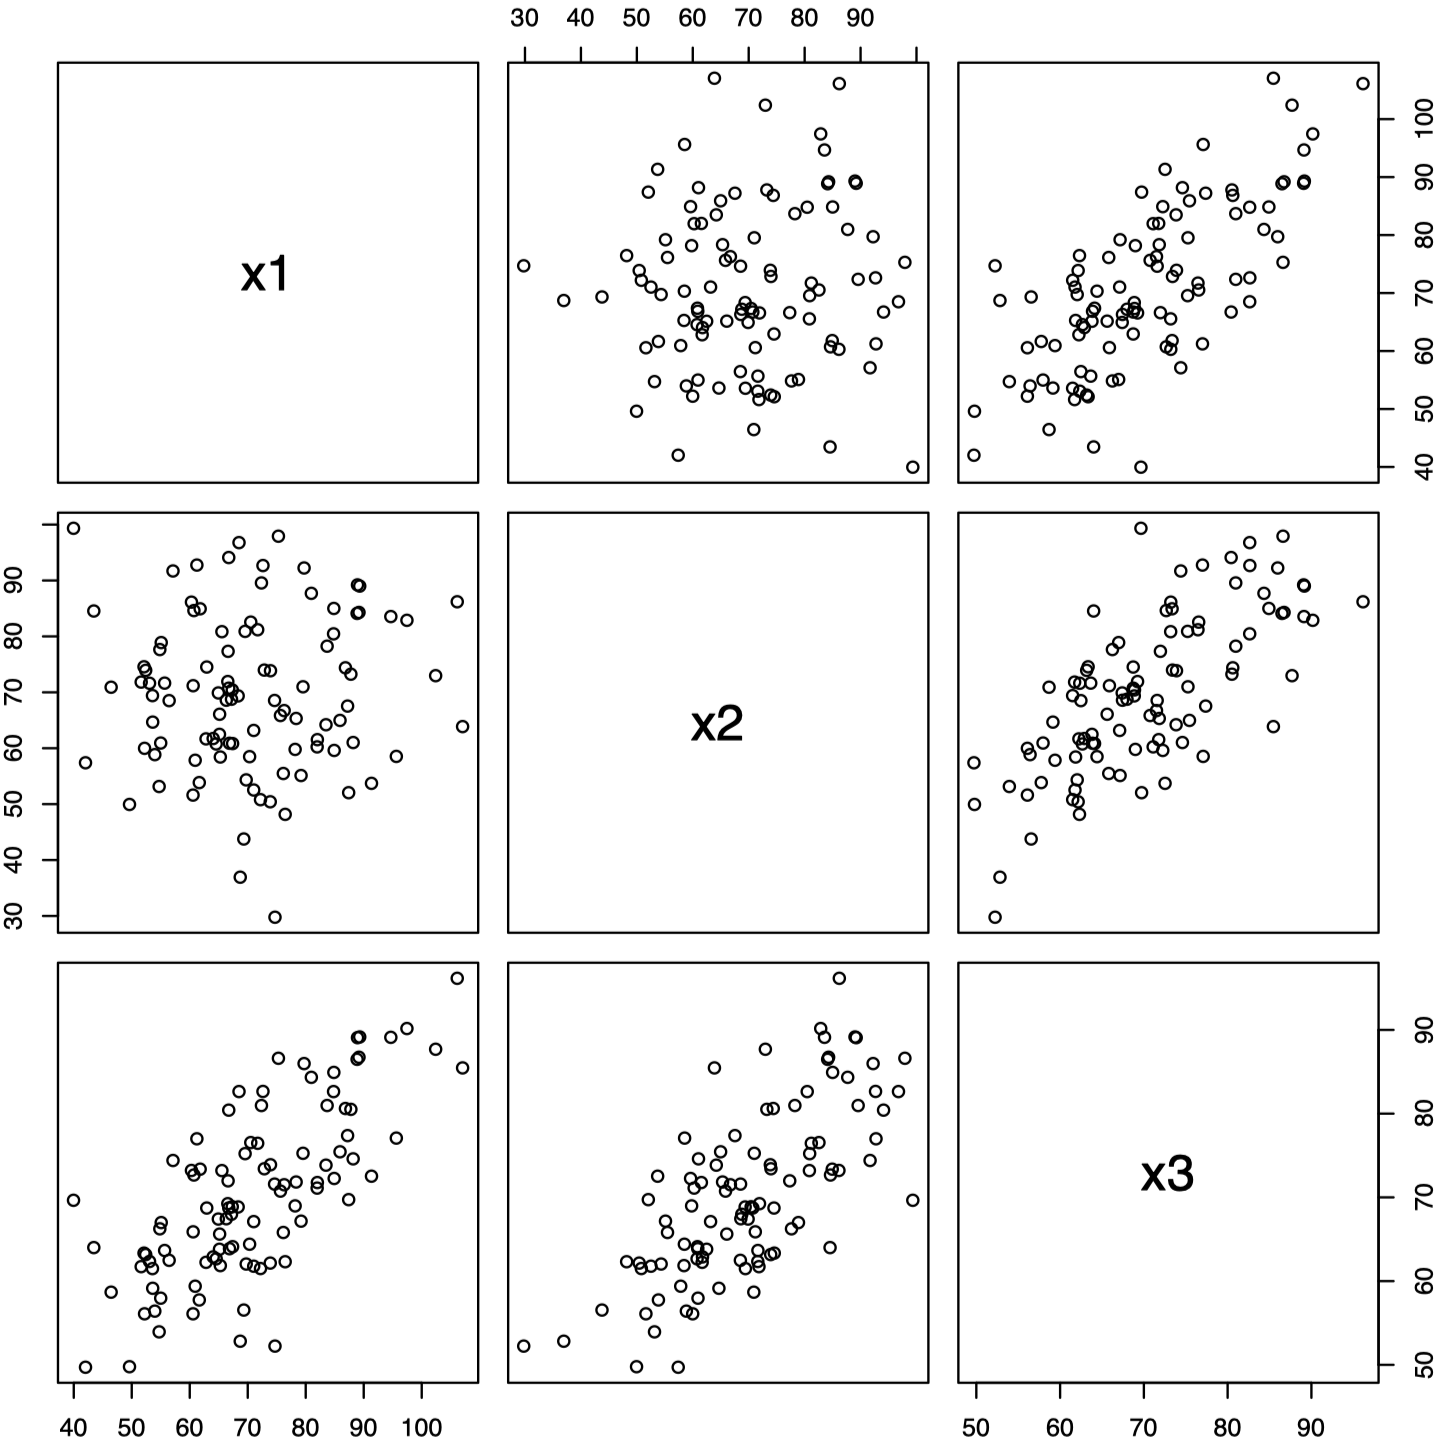
\includegraphics[width=6cm]{image01}
	\end{center}
	\caption{suppose $X_1$ and $X_2$ are independent Gaussians, of equal variance $\sigma^2$, and $X_3$ is their average,$X_3 = \left( X_1 + X_2 \right)/ 2$}
    \end{figure}
    \end{frame}
    
    
\section{Matrix-Geometric Perspective on Multicollinearity}
    \begin{frame}
    \frametitle{Multicollinearity}
    Multicollinearity means that
    \begin{equation*}
    	a_1X_1+a_2X_2+\hdots  a_pX_p=\sum_{i=1}^{p}a_iX_i=a_0
    \end{equation*}
    To simplify this, let's introduce p$\times$1 matrix
    \textbf{a} = $\begin{bmatrix}
	a_1
	\\a_2
	\\\vdots 
	\\a_p
    \end{bmatrix}$
    ,so we can write multicollinearity as    $\textbf{a}^{T} X = a_0$, for \textbf{a} $ \neq 0$
    \end{frame}
   
	\begin{frame}
	\begin{equation*}
	\begin{aligned}
	Var\left[ \textbf{a}^{T} X\right] &= 0,\quad \textbf{a} \neq 0
	\\\mbox{}
	\\Var\left[ \textbf{a}^{T} X\right] &= Var\left[ \sum_{i=1}^{p} a_i X_i\right]
	\\&=\sum_{i=1}^{p}\sum_{j=1}^{p}a_ia_j Cov\left[ X_i, X_j\right] 
	\\&=\textbf{a}^{T} Var\left[ X\right] \textbf{a}
	\end{aligned}
	\end{equation*}
    \end{frame}
	
	\begin{frame}
	\emph{•}The eigenvectors of Var[X], such that
	\begin{equation*}
		Var\left[ X\right] v_i=\lambda v_i
	\end{equation*}
	\\\emph{•}The eigenvalues are all ≥ 0.
	\\\emph{•}Any vector can be re-written as a sum of eigenvectors:
	\begin{equation*}
		\textbf{a}=\sum_{i=1}^{p}\left( \textbf{a}^{T} v_i\right) v_i
	\end{equation*}
	\\\emph{•}The eigenvectors can be chosen so that they all have length 1
	\\\quad and are orthogonal to each other.
	\\\emph{•}Var[X] can be expressed as 
	\begin{equation*}
		Var\left[ X\right] = VDV^{T}
	\end{equation*}
\end{frame}

	\begin{frame}
			\begin{equation*}
		\begin{aligned}
		Var\left[ X\right] \textbf{a} &= Var\left[ X\right]\sum_{i=1}^{p}\left( \textbf{a}^{T} v_i\right) v_i
		\\&=\sum_{i=1}^{p}\left( \textbf{a}^{T} v_i\right)Var\left[ X\right]v_i
		\\&=\sum_{i=1}^{p}\left( \textbf{a}^{T} v_i\right)\lambda_i v_i
		\\\textbf{a}^{T} Var\left[ X\right]\textbf{a}  
		&= \left( \sum_{i=1}^{p}\left( \textbf{a}^{T} v_i\right)v_j\right) ^{T} \sum_{i=1}^{p}\left( \textbf{a}^{T} v_i\right)\lambda_i v_i
		\\&=\sum_{i=1}^{p}\sum_{j=1}^{p}\left( \textbf{a}^{T} v_i\right)\left( \textbf{a}^{T} v_i\right)v_j^{T} v_i\lambda_i
		\\&=\sum_{i=1}^{p}\left( \textbf{a}^{T} v_i\right)^2\lambda_i
		\end{aligned}
		\end{equation*}
	\end{frame}
	\begin{frame}
	\emph{•}The predictors are multi-collinear if and only if Var[X] has  
	\\\quad zero eigenvalues.
	\\\mbox{}
	\\\emph{•}Every multi-collinear combination of the predictors is either 
	\\\quad an  eigenvector of Var[X] with zero eigenvalue, or a linear 
	\\\quad combination of such eigenvectors.
\end{frame}
\end{document}        